\section{Caratteristica volt-amperometrica di una lampadina}
Per eseguire l'analisi di un carico resistivo non ohmico abbiamo utilizzato come soggetto del test una lampadina. Sappiamo che, quando abbiamo davanti una resistenza che si comporta in modo ``ohmico'', il grafico della caratteristica volt-amperometrica è una retta passante per l'origine. Nel caso della lampadina, ci aspettiamo dunque una curva non lineare. Abbiamo sottoposto il circuito (identico a quello in Figura \ref{fig:circuiti}, con la lampadina al posto della resistenza Rx) a diversi valori di tensione fino a quello massimo di 12V. I risultati sono riportati nel grafico in Figura \ref{fig:lampadina}.

\begin{figure}[h]
    \centering
        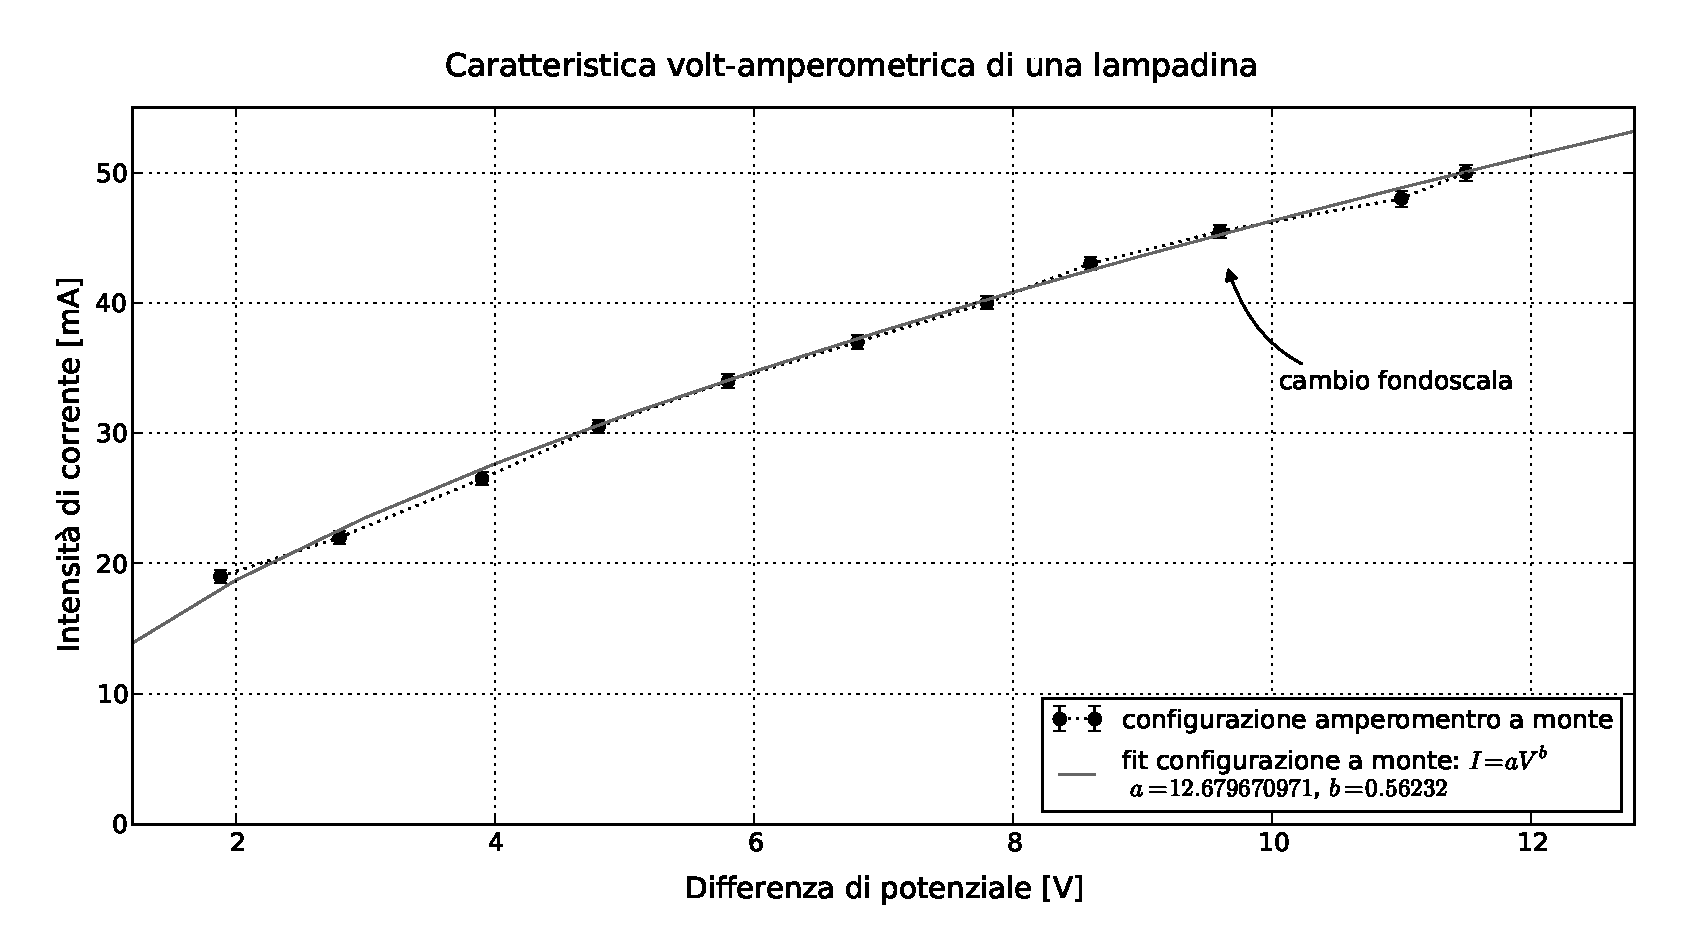
\includegraphics[width=\textwidth]{lamp.eps}
        \caption{Il grafico mostra la caratteristica volt-amperometrica di un carico resistivo non ohmico (lampadina).}
        \label{fig:lampadina}
\end{figure}

Si può notare che il circuito è sicuramente non ohmico, ma dai dati non risulta ovvia la funzione che definisce la caratteristica volt-amperomentrica della lampadina.

Abbiamo deciso di ipotizzare una legge del tipo $I=a \cdot V^{b}$. Proviamo una linearizzazione applicando $Log_{10}$ da entrambe le parti. Si ottiene dunque la relazione $Log_{10}I=b \cdot Log_{10}V + Log_{10}a$. Dal grafico riportato \footnote{E' stato eseguito il test del $\chi ^2_{exp}$, ottenendo come valore **, ampiamente compatibile con il valore teorico $\chi ^2_{teo}=** \pm **$ [intervallo di confidenza sul $\chi ^2_{teo}$ del 20\% ] } si vede come la linearizzazione sia stata efficace. I parametri stimati sono $a=** \pm **$ e $b=** \pm **$. 